\documentclass[preview]{standalone}

\usepackage{amsmath}
\usepackage{amssymb}
\usepackage{bettelini}
\usepackage{stellar}
\usepackage{tikz}
\usepackage{fancybox}
\usepackage{makecell}

\hypersetup{
    colorlinks=true,
    linkcolor=black,
    urlcolor=blue,
    pdftitle={Chimica},
    pdfpagemode=FullScreen,
}

\begin{document}

\title{Chimica}
\id{chimica-classificazione}
\genpage

\section{Definizione}

\begin{snippetdefinition}{sostanza-pura-elementare}{Sostanza pura elementare}
    Una \textit{sostanza pura elementare} è composta da un solo tipo di elemento.
\end{snippetdefinition}

\begin{snippetdefinition}{sostanza-pura-composta-definition}{Sostanza pura composta}
    Una \textit{sostanza pura composta} è composta da un solo tipo di composto.
\end{snippetdefinition}

\begin{snippetdefinition}{soluzione-definition}{Soluzione}
    Una \textit{soluzione} è una sostanza composta da diversi tipi di composti
    in maniera omogenea.
\end{snippetdefinition}

\begin{snippetexample}{sostanza-pura-composta-example}{Sostanza pura composta}
    Acqua (\(H_2O\))
\end{snippetexample}

\begin{snippetexample}{sostanza-pura-elementare-example}{Sostanza pura elementare}
    Azoto (\(N\))
\end{snippetexample}

\begin{snippetexample}{soluzione-example}{Soluzione}
    \(50\% N + 50\% H_2\)
\end{snippetexample}

\begin{snippet}{classificazione-sostanze-miscugli-illustrazione}
\begin{center}
    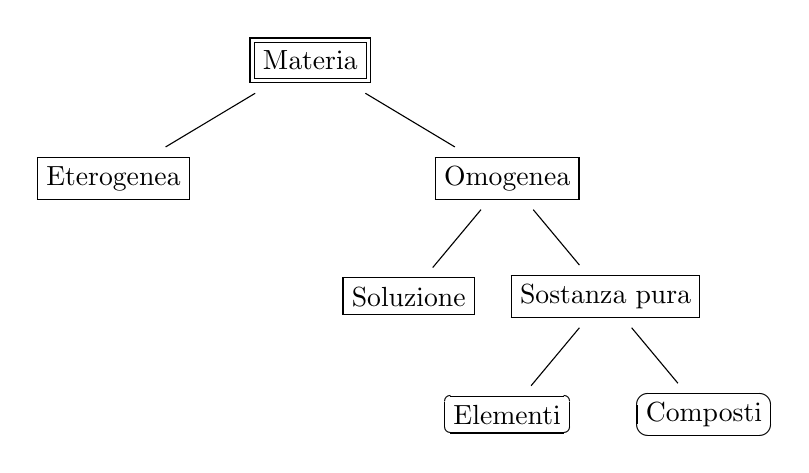
\begin{tikzpicture}[
        level 1/.style = {sibling distance = 5cm},
        level 2/.style = {sibling distance = 2.5cm}
    ]
    \node {\doublebox{Materia}}
        child {
            node {\fbox{Eterogenea}}
        }
        child {
            node {\fbox{Omogenea}}
            child {
                node {\fbox{Soluzione}}
            }
            child {
                node {\fbox{Sostanza pura}}
                child {
                    node {\ovalbox{Elementi}}
                }
                child {
                    node {\ovalbox{Composti}}
                }
            }
        };
    \end{tikzpicture}
\end{center}

\begin{itemize}
    \item La materia può essere classificata come materia \textit{eterogenea}
    e materia \textit{omogenea}.
    
    \item La materia omogenea può essere classificata come \textit{miscuglio omogeneo} (soluzione)
    oppure come \textit{sostanza pura}.
    
    \item Le sostanze pure possono essere classificati come \textit{elementi} oppure \textit{composti}.
\end{itemize}
\end{snippet}

\end{document}